\documentclass[11pt, a4paper]{article}

%====================================================================
% PREAMBLE (PENGATURAN DOKUMEN)
%====================================================================
\usepackage[T1]{fontenc}
\usepackage[english]{babel}
\usepackage{times}
\usepackage[utf8]{inputenc}
\usepackage{graphicx}
\usepackage{geometry}
\usepackage{fancyhdr}
\usepackage{booktabs}       % Untuk garis tabel yang profesional (toprule, midrule, bottomrule)
\usepackage{tabularx}       % <<< KUNCI UTAMA: Untuk tabel yang bisa text-wrapping
\usepackage{ragged2e}       % Untuk perataan teks yang lebih baik di kolom sempit
\usepackage{microtype}      % Untuk tipografi yang lebih baik, membantu mencegah overflow
\usepackage{hyperref}
\usepackage{tikz}
% \usepackage{fontawesome5}  % Commented out - not available

% --- Memuat library TikZ yang diperlukan ---
\usetikzlibrary{
    positioning,
    arrows.meta,
    shapes.geometric,
    shadows,
    backgrounds,
    calc,
    fit
}

% --- Definisi Kolom Baru untuk tabularx ---
% Kolom 'L' ini akan rata kiri dan teksnya otomatis turun baris (wrap)
\newcolumntype{L}{>{\RaggedRight\arraybackslash}X}

% --- Pengaturan Halaman ---
\geometry{a4paper, left=2.5cm, right=2.5cm, top=2.5cm, bottom=2.5cm}
\hypersetup{
    colorlinks=true,
    urlcolor=blue,
    linkcolor=black
}

% --- Pengaturan Header & Footer ---
\pagestyle{fancy}
\fancyhf{} % Hapus header/footer default
\fancyhead[L]{Proposal Hackathon: TalentMerit AI}
\fancyfoot[C]{\thepage}
\renewcommand{\headrulewidth}{0.4pt}
\renewcommand{\footrulewidth}{0.4pt}

\setlength{\headheight}{13.6pt} % Menambahkan ini untuk mengatasi warning dari fancyhdr


%====================================================================
% KONTEN DOKUMEN
%====================================================================
\begin{document}

%-------------------------------------------------
% HALAMAN JUDUL
%-------------------------------------------------
\begin{titlepage}
    \centering
    \vspace*{1cm}
    
    \Huge\bfseries
    PROPOSAL PROYEK HACKATHON
    
    \vspace{0.5cm}
    
    \huge\bfseries
    ASN DIGITAL AI HACKATHON 2025
    
    \vspace{2cm}
    
    \rule{\linewidth}{1.5pt}
    \vspace{0.4cm}
    \Huge\bfseries\textsc{TalentMerit AI}
    \newline
    \vspace{0.4cm}
    \large\textit{Ekosistem Meritokrasi Digital Berbasis Agentic AI dan Blockchain untuk Manajemen Talenta ASN}
    \vspace{0.4cm}
    \rule{\linewidth}{1.5pt}
    

    % perintah new line

    \vspace{3cm}
    
    \large
    \textbf{Nama Tim:} DFAI ANRI
    
    \vspace{0.5cm}
    
    \textbf{Anggota Tim:}
    
    \vspace{0.3cm}
    
    \begin{center}
        Tasdik Eko Pramono\\
        Jatniko Nur Mutaqin\\
        Rizal Aditya Herdianto
    \end{center}
    
    \vfill
    
    \large
    Oktober 2025
    
\end{titlepage}

\tableofcontents
\newpage

%-------------------------------------------------
% 1. JUDUL PROYEK
%-------------------------------------------------
\section{Judul Proyek}
\textbf{TalentMerit AI}: Ekosistem Meritokrasi Digital Berbasis Agentic AI dan Blockchain untuk Manajemen Talenta ASN.

%-------------------------------------------------
% 2. LATAR BELAKANG MASALAH
%-------------------------------------------------
\section{Latar Belakang Masalah}
Manajemen talenta di lingkungan Aparatur Sipil Negara (ASN) saat ini menghadapi tantangan fundamental yang menghambat terwujudnya birokrasi berkelas dunia. Sesuai dengan tema yang diangkat, yaitu \textbf{Sistem Meritokrasi dan Manajemen Talenta}, kami mengidentifikasi empat masalah utama:
\begin{enumerate}
    \item \textbf{Subjektivitas dalam Keputusan Karier:} Proses promosi, mutasi, dan penugasan seringkali masih dipengaruhi oleh faktor-faktor subjektif, yang dapat mencederai prinsip meritokrasi dan menurunkan motivasi ASN berprestasi.
    \item \textbf{Kesulitan Menemukan Talenta Internal:} Pimpinan unit kerja kesulitan mengidentifikasi ASN dengan kompetensi spesifik secara cepat dan akurat. Proses pencarian talenta masih bersifat manual dan tidak efisien.
    \item \textbf{Data Kompetensi yang Terfragmentasi:} Rekam jejak kinerja, keahlian, dan sertifikasi ASN tersebar, tidak terstandarisasi, dan sulit divalidasi, sehingga tidak dapat menjadi dasar pengambilan keputusan yang kuat.
    \item \textbf{Manajemen Talenta yang Reaktif:} Sistem HR saat ini cenderung menunggu adanya kebutuhan (reaktif), bukan secara proaktif memetakan talenta ke peluang strategis di masa depan.
\end{enumerate}
Masalah-masalah ini berujung pada penempatan talenta yang tidak optimal, kesenjangan kompetensi yang tidak terdeteksi, dan potensi ASN yang tidak termanfaatkan sepenuhnya.

%-------------------------------------------------
% 3. SOLUSI YANG DIUSULKAN
%-------------------------------------------------
\section{Solusi yang Diusulkan: TalentMerit AI}
Untuk menjawab tantangan tersebut, kami mengusulkan \textbf{TalentMerit AI}, sebuah platform revolusioner yang mentransformasi manajemen talenta ASN menjadi sebuah ekosistem yang proaktif, objektif, dan transparan. Solusi kami adalah sebuah aplikasi berbasis web yang ditenagai oleh \textbf{Agentic AI} dan diamankan oleh teknologi \textbf{Blockchain/Distributed Ledger Technology (DLT)}.

\subsection{Arsitektur dan Alur Kerja Sistem}
TalentMerit AI beroperasi sebagai sebuah siklus berkelanjutan yang ditenagai oleh teknologi canggih di setiap tahapnya, memastikan objektivitas dari hulu ke hilir.

\begin{figure}[h!]
    \centering
    % Menyesuaikan ukuran gambar agar tidak melebihi lebar teks
    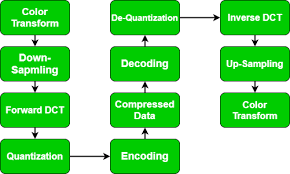
\includegraphics[width=0.9\textwidth]{download_image.png}
    \caption{Arsitektur dan Alur Kerja Sistem TalentMerit AI}
    \label{fig:arsitektur}
\end{figure}
\clearpage % <<< Tambahkan ini agar halaman selanjutnya tidak terganggu oleh posisi gambar

\subsection{Penerapan Teknologi}
\begin{itemize}
    \item \textbf{AI Agentic Core (Docling + LLM):} Teknologi AI canggih digunakan untuk (1) memahami struktur dokumen bukti kinerja melalui \textbf{Docling}, dan (2) melakukan validasi, penalaran, dan scoring secara kontekstual melalui \textbf{Large Language Model (LLM)}. Ini memastikan penilaian yang objektif dan mendalam.
    \item \textbf{AI Predictive Analytics:} Menganalisis data historis dari ledger untuk mengidentifikasi pola kinerja, memprediksi potensi keberhasilan ASN di jenjang berikutnya, dan memberikan rekomendasi promosi yang berbasis data.
    \item \textbf{Immutable Merit Ledger (Blockchain/DLT):} Setiap kinerja yang tervalidasi dicatat sebagai transaksi terenkripsi dalam sebuah \textit{distributed ledger}. Ini menciptakan rekam jejak yang \textbf{aman, transparan, dan tidak dapat diubah (immutable)}, memberantas potensi manipulasi data.
\end{itemize}
Solusi ini dapat segera direalisasikan dalam bentuk prototipe (MVP) aplikasi web yang fungsional selama periode hackathon.

%-------------------------------------------------
% 4. TARGET PENGGUNA
%-------------------------------------------------
\section{Target Pengguna}
Sistem ini dirancang untuk digunakan oleh seluruh lapisan kepegawaian negara, menciptakan ekosistem yang terintegrasi:
\begin{itemize}
    \item \textbf{ASN Aktif (Semua Jenjang):} Sebagai pengguna utama yang melaporkan bukti kinerja, membangun profil merit, dan mendapatkan rekomendasi pengembangan diri.
    \item \textbf{Pimpinan Unit Kerja (Eselon):} Sebagai pengambil keputusan yang menggunakan sistem untuk mencari talenta internal, mendapatkan rekomendasi kandidat untuk proyek/jabatan, dan menetapkan arah kinerja tim.
    \item \textbf{Manajemen Kepegawaian (BKN/BKPSDM):} Sebagai administrator dan analis strategis yang memantau peta kompetensi nasional/daerah, mengidentifikasi \textit{skill gap}, dan merancang kebijakan pengembangan talenta.
\end{itemize}

\newpage % <<< Tambahkan ini untuk kerapian tata letak
%-------------------------------------------------
% 5. KEUNGGULAN
%-------------------------------------------------
\section{Keunggulan Kompetitif}
\begin{itemize}
    \item \textbf{Objektivitas Maksimal:} Mengurangi bias manusia secara drastis dengan menyerahkan proses validasi dan scoring kepada AI Agent yang imparsial.
    \item \textbf{Sistem Proaktif, Bukan Reaktif:} AI secara mandiri memetakan talenta dengan peluang, memberikan rekomendasi sebelum diminta.
    \item \textbf{Transparansi dan Akuntabilitas Tinggi:} Teknologi Blockchain memastikan semua rekam jejak kinerja tercatat permanen, tidak dapat diubah, dan dapat diaudit.
    \item \textbf{Efisiensi Proses:} Mempercepat proses pencarian talenta dan suksesi jabatan dari hitungan minggu menjadi hitungan menit.
    \item \textbf{Membangun Budaya Kinerja:} Mendorong ASN untuk fokus pada kinerja yang terukur dan berdampak, karena setiap kontribusi positif akan dicatat dan dihargai secara sistematis.
\end{itemize}

%-------------------------------------------------
% 6. DAMPAK DAN POTENSI SKALA
%-------------------------------------------------
\section{Dampak dan Potensi Skala}
\textbf{Dampak} yang diharapkan dari implementasi TalentMerit AI sangat signifikan:
\begin{itemize}
    \item \textbf{Peningkatan Kualitas Tata Kelola:} Menempatkan ASN yang paling kompeten pada posisi yang tepat akan secara langsung meningkatkan kualitas layanan publik dan efektivitas program pemerintah.
    \item \textbf{Meningkatkan Motivasi dan Retensi Talenta:} ASN merasa dihargai berdasarkan kinerja nyata, meningkatkan kepuasan kerja dan loyalitas.
    \item \textbf{Pemberantasan KKN:} Transparansi total dari rekam jejak kinerja berbasis Blockchain secara efektif menutup celah untuk praktik korupsi, kolusi, dan nepotisme dalam manajemen karier.
\end{itemize}
\textbf{Potensi Skala} dari sistem ini sangat besar. Prototipe dapat diuji coba pada satu unit kerja atau instansi, kemudian dapat diskalakan untuk diadopsi oleh seluruh kementerian/lembaga/pemerintah daerah, hingga akhirnya menjadi sistem operasi manajemen talenta terpusat untuk seluruh ASN di Indonesia.

%-------------------------------------------------
% 7. RENCANA EKSEKUSI & TIMELINE
%-------------------------------------------------
\section{Rencana EkseKusi \& Timeline (Lingkup Hackathon)}
Kami akan fokus membangun prototipe (MVP) yang mendemonstrasikan alur kerja inti.
\begin{table}[h!]
    \centering
    \caption{Timeline Pengembangan Prototipe}
    % <<< PERBAIKAN DI SINI: Menggunakan tabularx >>>
    \begin{tabularx}{\textwidth}{@{} >{\bfseries}l L @{}}
        \toprule
        Waktu & Aktivitas Utama \\
        \midrule
        Hari 1 & \textbf{Desain Arsitektur:} Finalisasi Tech Stack (Python FastAPI, React, Ollama, LangChain). \\
               & \textbf{Backend:} Setup API endpoint untuk unggah dokumen dan profil pengguna. \\
               & \textbf{AI Setup:} Instalasi dan pengujian model LLM lokal melalui Ollama. \\
        \addlinespace
        Hari 2 & \textbf{AI Logic:} Implementasi \textit{Agentic chain} menggunakan LangChain untuk alur: Docling $\rightarrow$ LLM $\rightarrow$ JSON. \\
               & \textbf{Frontend:} Pengembangan UI untuk halaman profil, unggah dokumen, dan dasbor manajer. \\
               & \textbf{Database:} Desain skema database (SQLite) untuk menyimpan profil merit terstruktur. \\
        \addlinespace
        Hari 3 & \textbf{Integrasi:} Menghubungkan Frontend, Backend, dan AI Agent. Pengujian end-to-end. \\
               & \textbf{Demo Prep:} Mempersiapkan alur demo yang naratif dan visual, memastikan semua fitur MVP berjalan lancar. \\
               & \textbf{Finalisasi:} Polishing UI/UX dan penyelesaian materi presentasi. \\
        \bottomrule
    \end{tabularx}
\end{table}

%-------------------------------------------------
% 8. RENCANA ANGGARAN BIAYA (RAB)
%-------------------------------------------------
\section{Rencana Anggaran Biaya (RAB)}
Untuk lingkup Hackathon, pengembangan prototipe tidak memerlukan biaya karena kami akan menggunakan teknologi \textit{open-source} dan infrastruktur lokal. Namun, untuk implementasi skala penuh pasca-hackathon, estimasi biaya operasional bulanan adalah sebagai berikut:
\begin{table}[h!]
    \centering
    \caption{Estimasi Biaya Operasional Bulanan (Skala Penuh)}
    % <<< PERBAIKAN DI SINI: Menggunakan tabularx >>>
    \begin{tabularx}{\textwidth}{@{} l L r @{}}
        \toprule
        \textbf{No.} & \textbf{Komponen Biaya} & \textbf{Estimasi (IDR/Bulan)} \\
        \midrule
        1 & Cloud Infrastructure (Server, Database, Storage) & 15.000.000 \\
        2 & API LLM (Jika menggunakan model terkelola) & 7.500.000 \\
        3 & Biaya Maintenance \& Dukungan Teknis (1 FTE) & 12.000.000 \\
        4 & Lisensi Perangkat Lunak Pendukung & 2.500.000 \\
        \midrule
        \multicolumn{2}{r}{\textbf{Total Estimasi}} & \textbf{37.000.000} \\
        \bottomrule
    \end{tabularx}
    \caption*{\small \textit{Catatan: Biaya ini bersifat estimasi dan dapat disesuaikan tergantung skala pengguna dan pilihan teknologi final.}}
\end{table}

\end{document}